\documentclass[11pt]{amsart}
\usepackage[margin=1.15in]{geometry}
\usepackage[T1]{fontenc}
\usepackage{lmodern}
\usepackage{amssymb,amsmath,mathtools}
\usepackage{graphicx,float}
\usepackage[hidelinks]{hyperref}
\usepackage[expansion=false]{microtype}

\newtheorem{theorem}{Theorem}[section]
\newtheorem{proposition}[theorem]{Proposition}
\newtheorem{lemma}[theorem]{Lemma}
\newtheorem{corollary}[theorem]{Corollary}
\newtheorem{mainthm}{Theorem}
\renewcommand{\themainthm}{\Alph{mainthm}}
\theoremstyle{definition}
\newtheorem{definition}[theorem]{Definition}
\newtheorem{remark}[theorem]{Remark}
\newtheorem{example}[theorem]{Example}
\newtheorem*{question}{Question}

\newcommand{\ZZ}{\mathbb{Z}}
\newcommand{\QQ}{\mathbb{Q}}
\newcommand{\FF}{\mathbb{F}}
\newcommand{\PP}{\mathbb{P}}
\newcommand{\OO}{\mathcal{O}}
\DeclareMathOperator{\Res}{Res}
\DeclareMathOperator{\Pic}{Pic}
\DeclareMathOperator{\Spec}{Spec}
\newcommand{\zenodoCodeDOI}{10.5281/zenodo.XXXXXXXX}

\setlength{\emergencystretch}{2.5em}
\hbadness=2000
\raggedbottom
\begin{document}

\title[Isomorphic invariant orders without Hermite equivalence]{Isomorphic Invariant Orders\\ Without Hermite Equivalence}

\author{Deep Bhattacharjee}
\address{Formerly, Electro-Gravitational Space Propulsion Laboratory (EGSPL), Bhubaneswar, Odisha 751030, India}
\address{Formerly, University of Calcutta (Heramba Chandra College), 23/49 Gariahat Road, Golpark, Kolkata 700029, West Bengal, India}
\email{d.bhattacharjee@erl-forschung.de}
\email{itsdeep@live.com}
\email{egspl@proton.me (GitHub-related contact; GitHub account creelie)}
\urladdr{https://orcid.org/0000-0003-0466-750X}

\begin{abstract}
Bhargava, Evertse, Gy\H{o}ry, Remete and Swaminathan asked whether, in every degree $n\ge4$, there are integral polynomials with isomorphic invariant orders that are not Hermite equivalent; they answered the question for $n=4$. We answer it for every even $n$ and for every $n$ with $n-2$ divisible by $3$, $5$ or $7$, with explicit pairs. In degree six one polynomial of the pair can be chosen monic.

\medskip\noindent\textbf{Keywords:} Hermite equivalence; invariant order; binary form.

\smallskip\noindent\textbf{MSC 2020:} 11R04 (primary); 11C08, 11E16, 11R29.
\end{abstract}

\maketitle

\section{Introduction}\label{sec:intro}

In 1857 Hermite introduced an equivalence relation on integral polynomials of a given degree $n$ that is coarser than the classical $\mathrm{GL}_2(\ZZ)$-equivalence, and proved that there are only finitely many classes of a given nonzero discriminant. Bhargava, Evertse, Gy\H{o}ry, Remete and Swaminathan revived the notion and gave it an algebraic meaning \cite{BEGRS23}. To a polynomial
\[
f(X)=f_0X^n+f_1X^{n-1}+\dots+f_n\in\ZZ[X],\qquad f_0\neq0,\quad D(f)\neq0,
\]
one attaches its \emph{invariant order} $R_f$ and its \emph{invariant ideal} $I_f$, a fractional ideal of $R_f$; both live in the \'etale algebra $K_f=\QQ[X]/(f)$ and go back to Birch--Merriman, Nakagawa, Simon and Wood \cite{BM72,Nak89,Sim01,Woo11}. For primitive $f$ and $g$ of nonzero discriminant, $f$ and $g$ are Hermite equivalent if and only if there is a ring isomorphism $R_f\cong R_g$ under which the ideal classes of $I_f$ and $I_g$ correspond \cite[Corollary~3.12]{BEGRS23}. In degree three the condition on ideals is automatic, by the Levi--Delone--Faddeev correspondence, and for monic polynomials it is empty, since then $I_f=R_f$. This led the authors to the following question.\footnote{Question 3.18 of \cite{BEGRS23}. We quote it in full.}

\begin{question}[Bhargava--Evertse--Gy\H{o}ry--Remete--Swaminathan]
Let $n\ge4$. Do there exist (reducible or irreducible) polynomials $f,g\in\ZZ[X]$ of degree $n$ and nonzero discriminant that have isomorphic invariant orders but are not Hermite equivalent, and if so, can such polynomials be exhibited?
\end{question}

In \cite[Theorem~3.20]{BEGRS23} they exhibited two quartic polynomials with isomorphic invariant orders, one with principal and one with non-principal invariant ideal, which settles $n=4$. For $n\ge5$ the question has remained open. Our main result settles it in most degrees.

\begin{mainthm}\label{thm:A}
Let $n\ge5$ and suppose that $n$ is even or that $n-2$ is divisible by $3$, $5$ or $7$. Then there exist primitive polynomials $P,P'\in\ZZ[X]$ of degree $n$ and the same nonzero discriminant whose invariant orders are isomorphic and which are not Hermite equivalent. For $n\ge6$ there are infinitely many such pairs with pairwise distinct discriminants.
\end{mainthm}

Together with the quartic case, the question is answered for every $n\ge4$ except the odd $n$ for which $n-2$ is prime to $105$; the first of these are $13,15,19,21,25$ (Figure~\ref{fig:degrees}). In the two smallest degrees the pairs are short enough to write down.

\begin{mainthm}\label{thm:B}
The sextic polynomials
\begin{align*}
P(X)&=X^6-18X^4-6X^3+79X^2+60X+10,\\
P'(X)&=3X^6+8X^5-22X^4-82X^3-67X^2-20X-2
\end{align*}
have the same discriminant and isomorphic invariant orders, and they are not Hermite equivalent. The same holds for the quintic polynomials
\begin{align*}
Q(X)&=14X^5-19X^4-1676X^3+3714X^2+50843X-152646,\\
Q'(X)&=42X^5-169X^4-2608X^3+12820X^2+975X-45526.
\end{align*}
\end{mainthm}

The sextic $P$ is monic. By \cite[Corollary~3.16]{BEGRS23} two monic polynomials with isomorphic invariant orders are always Hermite equivalent, so Theorem~\ref{thm:B} shows that this statement fails as soon as only one of the two polynomials is monic.

The idea behind both theorems is simple. Take two binary quadratic forms $q_0$ and $q_1$ of the same discriminant $d$, so that their invariant orders coincide, with $I_{q_0}$ principal and $I_{q_1}$ not. A single binary form $H$ that is coprime to both $q_0$ and $q_1$ at every prime, in the sense that $\Res(q_0,H)=\Res(q_1,H)=\pm1$, splits off a common factor: the invariant order of $q_iH$ is the product of the invariant orders of $q_i$ and $H$, and the invariant ideal splits in the same way. The two products then have the same ring but invariant ideals that differ in exactly one factor, and a count of the principal factors shows that no isomorphism can identify them. The whole difficulty is to find such an $H$ in the required degree. Section~\ref{sec:exist} shows that the obstruction lives in the Picard group of the quartic ring attached to $q_0q_1$, and that one form of degree $k$ produces forms in every degree divisible by $k$. Section~\ref{sec:data} gives the four quadratic fields and the five forms that prove Theorem~\ref{thm:A}.

\begin{figure}[H]
\centering
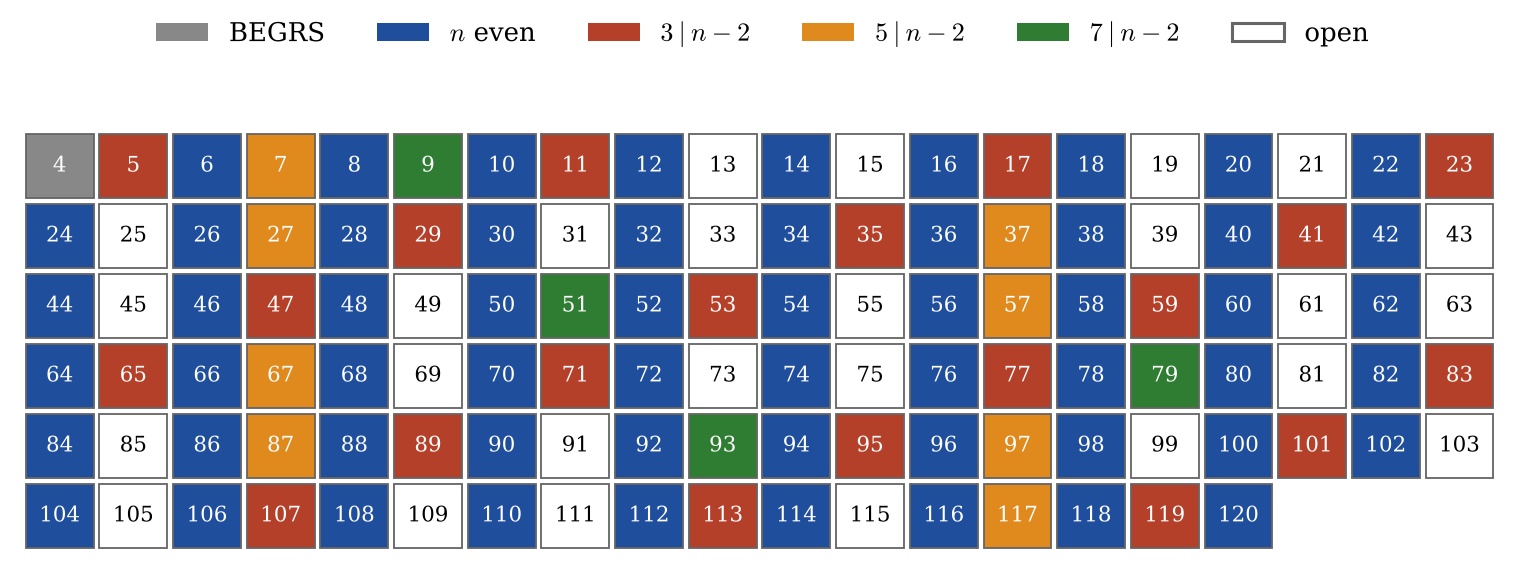
\includegraphics[width=0.95\textwidth]{fig_degrees.png}
\caption{Degrees $4\le n\le120$ in which Question~3.18 of \cite{BEGRS23} is answered. Grey: the quartic example of \cite{BEGRS23}. Coloured: Theorem~\ref{thm:A}, by the first divisibility condition it satisfies. White: degrees left open.}
\label{fig:degrees}
\end{figure}

\section{Invariant orders, invariant ideals and resultants}\label{sec:prelim}

We identify a polynomial $f\in\ZZ[X]$ of degree $n$ with the binary form $f(x,y)=y^nf(x/y)$ and use the same letter for both. Throughout, $f_0=f(1,0)\neq0$ and $D(f)\neq0$. Let $\alpha$ be the image of $X$ in $K_f=\QQ[X]/(f)$. The $\ZZ$-module $I_f(k)\subset K_f$, for $0\le k\le n-1$, has basis
\[
1,\ \alpha,\ \dots,\ \alpha^k,\ \zeta_{k+1},\ \dots,\ \zeta_{n-1},\qquad \zeta_i=f_0\alpha^i+f_1\alpha^{i-1}+\dots+f_{i-1}\alpha,
\]
and $R_f=I_f(0)$, $I_f=I_f(1)$ \cite[\S3.1]{BEGRS23}. We use four facts from \cite[Theorem~3.3]{BEGRS23}, due to Birch--Merriman, Nakagawa, Simon and Wood:

\begin{enumerate}
\item[(F1)] $R_f$ is an order in $K_f$ and $D(R_f)=D(f)$.
\item[(F2)] $I_f(k)$ is a fractional ideal of $R_f$; it is invertible if and only if $f$ is primitive, and then $I_f(k)=I_f^k$.
\item[(F3)] Let $S_f\subset\PP^1_\ZZ$ be the closed subscheme cut out by $f$. Then $R_f$ is the ring of global functions on $S_f$ and $I_f(k)$ is the module of global sections of $\OO(k)|_{S_f}$. Both are viewed inside $K_f$ through the generic fibre $S_f\times\QQ=\Spec K_f$, sections of $\OO(k)$ being divided by $y^k$.
\item[(F4)] Primitive $f,g$ of degree $n$ and nonzero discriminant are Hermite equivalent if and only if there is a ring isomorphism $\varphi\colon R_f\to R_g$ with $\varphi(I_f)$ in the ideal class of $I_g$ \cite[Corollary~3.12]{BEGRS23}.
\end{enumerate}

Statement (F3) is Wood's geometric description \cite[\S2 and Appendix~A]{Woo11}.\footnote{Wood works over an arbitrary base scheme and also treats forms of discriminant zero; we only need the case of integral forms with $f_0D(f)\neq0$, where $S_f$ is finite and flat over $\Spec\ZZ$.} The identification inside $K_f$ uses that $f_0\neq0$, so the generic fibre of $S_f$ lies in the chart $y\neq0$, where it is $\Spec\QQ[t]/(f(t,1))$; the section $x^jy^{k-j}$ goes to $\alpha^j$.

For a binary quadratic form $q=ax^2+bxy+cy^2$ of non-square discriminant $d=b^2-4ac$ with $a\neq0$, let $\theta=(-b+\sqrt d)/(2a)$. Then $K_q=\QQ(\sqrt d)$, $R_q=\ZZ+\ZZ a\theta=\ZZ[(d+\sqrt d)/2]$ is the quadratic order $\OO_d$ of discriminant $d$, and $I_q=\ZZ+\ZZ\theta$. In particular two quadratic forms of the same discriminant have literally the same invariant order. If $q$ is primitive, then $aI_q=\ZZ a+\ZZ\tfrac{-b+\sqrt d}{2}$ is the invertible ideal of norm $|a|$ classically attached to $q$. If $a=1$ then $I_q=R_q$ is principal.

For binary forms $F,G$ of degrees $a,b\ge1$ we write $\Res(F,G)$ for their resultant. We need the following standard properties \cite[Chapter~IV, \S8 and Chapter~IX, \S3]{Lan02}.

\begin{lemma}\label{lem:res}
Let $F,G,G_1,G_2,M$ be integral binary forms with $\deg F=a$, $\deg G=b$ and $\deg M=b-a\ge0$.
\begin{enumerate}
\item $\Res(F,G)=\pm1$ if and only if $F$ and $G$ have no common zero in $\PP^1(\overline{\FF}_p)$ for any prime $p$.
\item $\Res(F,G_1G_2)=\Res(F,G_1)\Res(F,G_2)$ and $\Res(F,cG)=c^a\Res(F,G)$ for $c\in\ZZ$.
\item $\Res(F,G+FM)=\Res(F,G)$.
\item $D(FG)=D(F)D(G)\Res(F,G)^2$.
\end{enumerate}
\end{lemma}

\begin{proof}
The resultant of binary forms is a universal integral polynomial in the coefficients, so it commutes with reduction modulo $p$, and over an algebraically closed field it vanishes exactly when the two forms have a common zero in $\PP^1$. Since $\Res(F,G)$ is an integer, it equals $\pm1$ if and only if it is not divisible by any prime, which is (1). If $F=f_0\prod_{i=1}^a(x-\alpha_iy)$ with $f_0\neq0$, then $\Res(F,G)=f_0^{\,b}\prod_iG(\alpha_i,1)$ up to a sign depending only on $a$ and $b$; this gives (2) and (3), because $FM$ vanishes at every $(\alpha_i,1)$. The general case of (2) and (3) follows by continuity in the coefficients, or by a change of variables in $\mathrm{GL}_2(\ZZ)$ that makes $F(1,0)\neq0$. Part (4) is the usual product formula for discriminants.
\end{proof}

\section{Splitting off a common factor}\label{sec:split}

\begin{lemma}\label{lem:split}
Let $F$ and $G$ be primitive binary forms of degrees $a,b\ge2$ with nonzero leading coefficients $F(1,0)$, $G(1,0)$, nonzero discriminants, and $\Res(F,G)=\pm1$. Then the isomorphism of $\QQ$-algebras
\[
K_{FG}\longrightarrow K_F\times K_G,\qquad X\longmapsto(\alpha_F,\alpha_G),
\]
given by the Chinese remainder theorem maps $R_{FG}$ onto $R_F\times R_G$ and $I_{FG}$ onto $I_F\times I_G$.
\end{lemma}

\begin{proof}
On the affine chart $y\neq0$ of $\PP^1_\ZZ$ the schemes $S_F$, $S_G$ and $S_{FG}$ are cut out by $F(t,1)$, $G(t,1)$ and their product in $\ZZ[t]$. By Lemma~\ref{lem:res}(1) the scheme $\Spec\ZZ[t]/(F(t,1),G(t,1))$ has no points, so the two ideals are comaximal. For comaximal ideals the intersection equals the product, and the Chinese remainder theorem gives
\[
\ZZ[t]/\bigl(F(t,1)G(t,1)\bigr)\cong\ZZ[t]/\bigl(F(t,1)\bigr)\times\ZZ[t]/\bigl(G(t,1)\bigr).
\]
The same holds on the chart $x\neq0$. Hence $S_{FG}$ is the disjoint union of its closed subschemes $S_F$ and $S_G$, and global sections of $\OO(k)$ on $S_{FG}$ are pairs of global sections on $S_F$ and on $S_G$. On the generic fibre this decomposition is the map in the statement, since $\QQ[t]/(F(t,1)G(t,1))\cong\QQ[t]/(F(t,1))\times\QQ[t]/(G(t,1))$ sends $t$ to $(\alpha_F,\alpha_G)$, and dividing by $y^k$ commutes with it. Apply (F3) with $k=0$ and $k=1$; the latter is allowed because $a,b\ge2$.
\end{proof}

\begin{figure}[H]
\centering
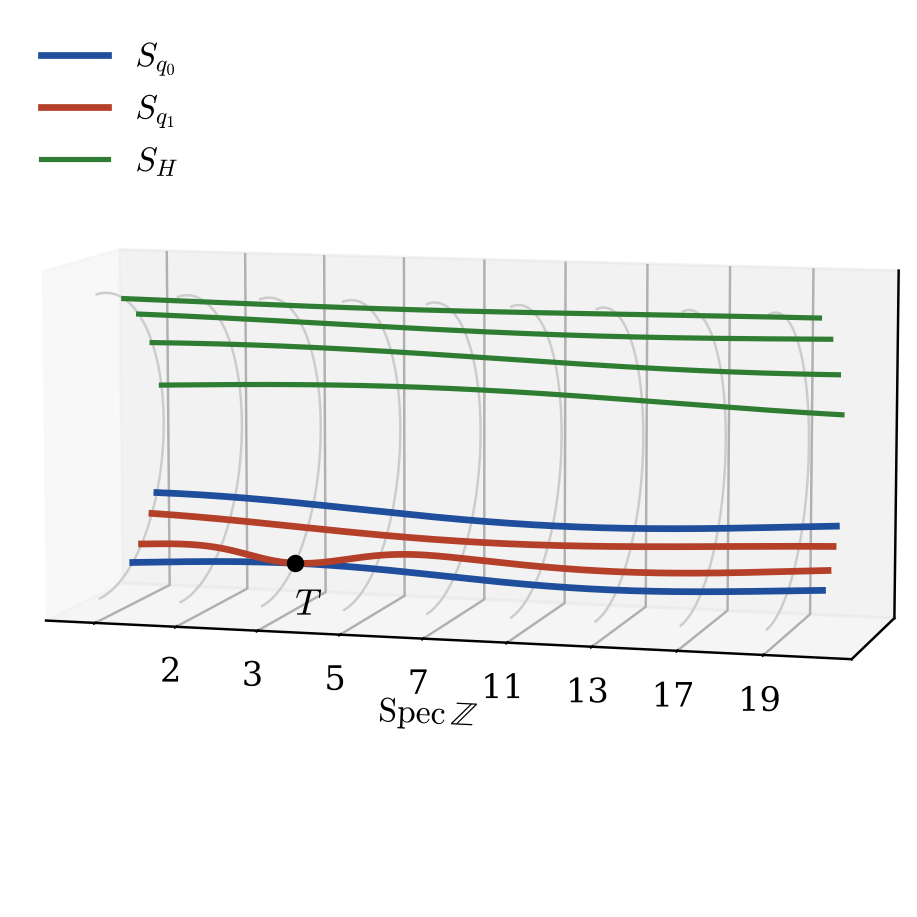
\includegraphics[width=0.78\textwidth]{fig_scheme.png}
\caption{A schematic picture of $\PP^1_\ZZ\to\Spec\ZZ$. The subschemes $S_{q_0}$ and $S_{q_1}$ of two quadratic forms of the same discriminant always meet, here over a single prime, in a finite scheme $T$. Theorem~\ref{thm:twist} needs a form $H$ whose subscheme $S_H$ avoids both of them in every fibre.}
\label{fig:scheme}
\end{figure}

\section{The twisting principle}\label{sec:twist}

\begin{theorem}\label{thm:twist}
Let $q_0$ and $q_1$ be primitive binary quadratic forms of the same non-square discriminant $d$ with $q_0(1,0)q_1(1,0)\neq0$, such that $I_{q_0}$ is a principal ideal of $\OO_d$ and $I_{q_1}$ is not. Let $H$ be a binary form of degree $k\ge2$ with $H(1,0)D(H)\neq0$ and
\[
\Res(q_0,H)=\pm1,\qquad\Res(q_1,H)=\pm1.
\]
Then $P=q_0H$ and $P'=q_1H$ are primitive of degree $k+2$, $D(P)=D(P')=d\,D(H)\neq0$, $R_P\cong R_{P'}$, and $P$ and $P'$ are not Hermite equivalent.
\end{theorem}

\begin{proof}
If a prime $\ell$ divided every coefficient of $H$, then $\ell^2$ would divide $\Res(q_0,H)$ by Lemma~\ref{lem:res}(2). So $H$ is primitive, and $P$, $P'$ are primitive by Gauss's lemma. Their leading coefficients $q_i(1,0)H(1,0)$ are nonzero, and Lemma~\ref{lem:res}(4) gives $D(P)=D(P')=d\,D(H)$, which is nonzero.

By Lemma~\ref{lem:split}, applied to $(q_0,H)$ and to $(q_1,H)$,
\[
R_P\cong\OO_d\times R_H\cong R_{P'},\qquad I_P\leftrightarrow I_{q_0}\times I_H,\qquad I_{P'}\leftrightarrow I_{q_1}\times I_H .
\]
Suppose that $P$ and $P'$ were Hermite equivalent. By (F4) there is a ring isomorphism $\varphi\colon R_P\to R_{P'}$ and $\kappa\in K_{P'}^\times$ with $\varphi(I_P)=\kappa I_{P'}$.

The order $R_H$ lies in the reduced algebra $K_H$, so it has finitely many idempotents, and it is the product of the rings $eR_H$ over its primitive idempotents $e$; each $eR_H$ has no idempotents other than $0$ and $e$. The primitive idempotents of $R_P=\OO_d\times R_H$ are $(1,0)$ and the $(0,e)$, because $\OO_d$ is a domain. A ring isomorphism sends primitive idempotents bijectively to primitive idempotents, and for each primitive idempotent $\varepsilon$ of $R_P$ it restricts to an isomorphism $\varepsilon R_P\to\varphi(\varepsilon)R_{P'}$ carrying $\varepsilon I_P$ onto $\varphi(\varepsilon)\kappa I_{P'}$, a principal multiple of $\varphi(\varepsilon)I_{P'}$.

For a ring $A$ with an ideal $J$ write $N(A,J)$ for the number of primitive idempotents $\varepsilon$ of $A$ such that $\varepsilon A$ is isomorphic to $\OO_d$ and $\varepsilon J$ is a principal ideal of $\varepsilon A$. The previous paragraph shows $N(R_P,I_P)=N(R_{P'},I_{P'})$. On the other hand the component $(1,0)$ contributes $1$ to $N(R_P,I_P)$, because $I_{q_0}$ is principal, and $0$ to $N(R_{P'},I_{P'})$, because $I_{q_1}$ is not; whether an ideal of $\OO_d$ is principal does not depend on the choice of isomorphism, since $\OO_d$ has only the identity and conjugation as automorphisms. The components $(0,e)$ contribute the same amount to both counts, because they carry the same pair $(eR_H,eI_H)$. Hence $N(R_P,I_P)=N(R_{P'},I_{P'})+1$, a contradiction.
\end{proof}

\begin{remark}\label{rem:class}
The proof uses only that $I_{q_0}$ and $I_{q_1}$ lie in different orbits of $\Pic(\OO_d)$ under conjugation. The principal case is the most convenient, because then $q_0$ can be taken monic.
\end{remark}

\section{Finding the common factor}\label{sec:exist}

Fix $q_0,q_1$ as in Theorem~\ref{thm:twist} and call a binary form $H$ \emph{admissible} if $\Res(q_0,H)=\pm1$ and $\Res(q_1,H)=\pm1$. Admissibility is stable under products and under adding multiples of $q_0q_1$.

\begin{proposition}\label{prop:family}
Let $H_1,\dots,H_s$ be admissible forms of degrees $k_1,\dots,k_s$, let $m_1,\dots,m_s\ge0$, and suppose $k=\sum m_jk_j\ge4$. Put $M=\prod_{i=1}^{k-4}(x-iy)$ and
\[
H_t=\prod_{j=1}^sH_j^{m_j}+t\,q_0q_1M\qquad(t\in\ZZ).
\]
Then every $H_t$ is admissible of degree $k$, and $H_t(1,0)D(H_t)\neq0$ for all but finitely many $t$. The values $D(H_t)$ are not all equal.
\end{proposition}

\begin{proof}
Admissibility of $H_t$ follows from Lemma~\ref{lem:res}(2) and (3), since $q_0q_1M$ is divisible by $q_0$ and by $q_1$. The leading coefficient $H_t(1,0)$ is a polynomial of degree one in $t$ with slope $q_0(1,0)q_1(1,0)\neq0$. The discriminant is homogeneous of degree $2k-2$ in the coefficients, so $D(H_t)$ is a polynomial in $t$ of degree at most $2k-2$ whose coefficient of $t^{2k-2}$ is
\[
D(q_0q_1M)=D(q_0)\,D(q_1)\,D(M)\,\Res(q_0,q_1)^2\,\Res(q_0,M)^2\,\Res(q_1,M)^2 .
\]
This is nonzero: $q_0$ and $q_1$ are irreducible over $\QQ$ and not proportional, because their invariant ideals are not in the same class; $M$ splits into distinct rational linear factors. Hence $D(H_t)$ is a nonconstant polynomial in $t$, which vanishes for finitely many $t$ only and takes infinitely many values.
\end{proof}

The next statement explains when admissible forms exist. It is not needed for the proof of Theorem~\ref{thm:A}, but it is how the forms in Section~\ref{sec:data} were found, and it shows what goes wrong in the remaining degrees.

\begin{proposition}\label{prop:criterion}
Let $F=q_0q_1$ and $k\ge3$. An admissible form of degree $k$ exists if and only if $I_F^k$ is a principal ideal of the quartic order $R_F$.
\end{proposition}

\begin{proof}
By Lemma~\ref{lem:res}(1),(2) a form $H$ of degree $k$ is admissible if and only if $H$ has no zero on $S_F$, that is, if and only if the section $H|_{S_F}$ of the invertible sheaf $\OO(k)|_{S_F}$ vanishes nowhere. Since $S_F$ is affine, this holds if and only if $H|_{S_F}$ generates the module of global sections, which is $I_F^k$ by (F2) and (F3); for $k\ge4$ one uses that $\OO(k)|_{S_F}$ is the $k$-th tensor power of the invertible sheaf $\OO(1)|_{S_F}$, whose module of sections $I_F$ is invertible, so that the sections form $I_F^{\otimes k}=I_F^k$. So an admissible $H$ makes $I_F^k$ principal. Conversely, the sequence $0\to\OO(k-4)\xrightarrow{\,F\,}\OO(k)\to\OO(k)|_{S_F}\to0$ on $\PP^1_\ZZ$ and the vanishing of $H^1(\PP^1_\ZZ,\OO(k-4))$ for $k\ge3$ \cite[Theorem~III.5.1]{Har77} show that every global section of $\OO(k)|_{S_F}$ is the restriction of a form of degree $k$. A generator of $I_F^k$ is therefore the restriction of an admissible form.
\end{proof}

The class of $I_F$ maps to $(1,[I_{q_1}])$ under $\Pic(R_F)\to\Pic(\OO_d)^2$, so $I_F^k$ can be principal only if $[I_{q_1}]^k=1$. The kernel of that map is $\OO_T^\times$ modulo the images of the two unit groups, where $\OO_T$ denotes the ring of functions on the finite scheme $T=S_{q_0}\cap S_{q_1}$ (Figure~\ref{fig:scheme}). The order of $I_F$ can therefore be larger than that of $[I_{q_1}]$, and it depends on the chosen forms within their classes; a large unit group helps, which is why all our examples come from real quadratic fields. Since an admissible form of degree $n-2$ forces $[I_{q_1}]^{n-2}=1$ while $[I_{q_1}]\neq1$, an odd degree $n$ always needs a quadratic order whose class group has an element of odd order dividing $n-2$.

\section{Four quadratic fields}\label{sec:data}

Table~\ref{tab:data} lists four pairs $(q_0,q_1)$. In each case $q_0$ is monic, so $I_{q_0}=\OO_d$ is principal. The discriminant $d$ is fundamental, $\OO_d$ is the full ring of integers of $\QQ(\sqrt d)$, and the class number $h$ is given for orientation only.

\begin{table}[H]
\centering
\renewcommand{\arraystretch}{1.25}
\begin{tabular}{ccccc}
$d$ & $h$ & $q_0$ & $q_1$ & admissible base forms\\\hline
$40$ & $2$ & $x^2-10y^2$ & $2x^2+4xy-3y^2$ & $H_4$, $H_6$\\
$229$ & $3$ & $x^2+xy-57y^2$ & $3x^2-5xy-17y^2$ & $H_3$\\
$401$ & $5$ & $x^2+xy-100y^2$ & $2x^2+23xy+16y^2$ & $H_5$\\
$577$ & $7$ & $x^2+xy-144y^2$ & $2x^2-11xy-57y^2$ & $H_7$
\end{tabular}
\caption{The quadratic data. The base forms are listed in the appendix.}
\label{tab:data}
\end{table}

\begin{lemma}\label{lem:nonprincipal}
In each row of Table~\ref{tab:data} the ideal $I_{q_1}$ is not principal.
\end{lemma}

\begin{proof}
Write $q_1=ax^2+bxy+cy^2$. By Section~\ref{sec:prelim}, $aI_{q_1}=\ZZ a+\ZZ\frac{-b+\sqrt d}{2}$ is an ideal $\mathfrak p$ of norm $a$, which is the prime $2$ or $3$. If $\mathfrak p$ were principal, $\pm a$ would be the norm of an element of $\OO_d$ not divisible by any rational integer, so $\pm a$ would be primitively represented by the principal form $q_0$.

For $d=40$ this is impossible modulo $5$: $x^2-10y^2\equiv x^2\pmod5$, and $\pm2$ are not squares modulo $5$.

For the other three rows we use reduction theory of indefinite forms \cite[Chapter~3]{Bue89}. A form $(A,B,C)$ of discriminant $d>0$ is reduced if $0<B<\sqrt d$ and $\sqrt d-B<2|A|<\sqrt d+B$; two reduced forms are equivalent if and only if they lie on the same cycle. If $m$ is primitively represented by $q_0$ and $|m|<\sqrt d/2$, then $q_0$ is equivalent to a form $(m,B,C)$, and replacing $B$ by its representative modulo $2|m|$ in the interval $(\sqrt d-2|m|,\sqrt d)$ makes it reduced. So $\pm a$ would appear as a first coefficient on the cycle of $q_0$. Here $a<\sqrt d/2$ in all three cases ($\sqrt d/2>7.5$), and the cycles of the principal forms are
\begin{align*}
d=229:&\quad(1,15,-1),\ (-1,15,1);\\
d=401:&\quad(1,19,-10),\ (-10,1,10),\ (10,19,-1),\ (-1,19,10),\ (10,1,-10),\ (-10,19,1);\\
d=577:&\quad(1,23,-12),\ (-12,1,12),\ (12,23,-1),\ (-1,23,12),\ (12,1,-12),\ (-12,23,1).
\end{align*}
Each step $(A,B,C)\mapsto(C,B',C')$ chooses $B'\equiv-B\pmod{2|C|}$ in $(\sqrt d-2|C|,\sqrt d)$, and one checks $B'^2-4CC'=d$ directly. The first coefficients are $\pm1$ for $d=229$ and $\pm1,\pm10$, resp.\ $\pm1,\pm12$, for $d=401$, $577$. Neither $\pm3$ nor $\pm2$ occurs.
\end{proof}

\begin{lemma}\label{lem:base}
The forms $H_4,H_6$ (for $d=40$), $H_3$ (for $d=229$), $H_5$ (for $d=401$) and $H_7$ (for $d=577$) listed in the appendix are admissible for the corresponding pair $(q_0,q_1)$, have nonzero leading coefficient and nonzero discriminant, and are irreducible over $\QQ$.
\end{lemma}

\begin{proof}
For each base form $H$ and each $i$ the number $\Res(q_i,H)$ is the determinant of an integer Sylvester matrix of size $\deg H+2$; equivalently, with $q_i=a_ix^2+b_ixy+c_iy^2$ and $\theta_i=(-b_i+\sqrt d)/(2a_i)$, it equals $a_i^{\deg H}N_{\QQ(\sqrt d)/\QQ}\bigl(H(\theta_i,1)\bigr)$. These finite computations give the values in the appendix, all equal to $\pm1$. Irreducibility and $D(H)\neq0$ are again finite checks; irreducibility is not used below.
\end{proof}

\begin{proof}[Proof of Theorem~\ref{thm:A}]
Let $n\ge5$ and $k=n-2\ge3$. If $n$ is even, write $k=4a+6b$ with $a,b\ge0$ and use the row $d=40$ with $H_4,H_6$. If $3\mid k$, $5\mid k$ or $7\mid k$, use the row $d=229$, $401$ or $577$ with the single base form $H_3$, $H_5$ or $H_7$ and exponent $k/3$, $k/5$ or $k/7$. If $k$ equals the degree of the base form, take $H$ to be that form; it is admissible with $H(1,0)D(H)\neq0$ by Lemma~\ref{lem:base}. Otherwise $k\ge4$, and Proposition~\ref{prop:family} gives admissible $H_t$ of degree $k$ with $H_t(1,0)D(H_t)\neq0$ for all but finitely many $t$, and with infinitely many distinct discriminants. By Lemma~\ref{lem:nonprincipal}, Theorem~\ref{thm:twist} applies to $P=q_0H$ and $P'=q_1H$. Their common discriminant $d\,D(H_t)$ takes infinitely many values as $t$ varies, which proves the last assertion; $k\ge4$ holds for every $n\ge6$.
\end{proof}

\begin{proof}[Proof of Theorem~\ref{thm:B}]
For the sextic pair take $d=40$, $q_0=x^2-10y^2$, the form $q_1^\ast=3x^2+8xy+2y^2$ of discriminant $40$, and $H=x^4-8x^2y^2-6xy^3-y^4$. Then $P=q_0H$ and $P'=q_1^\ast H$, and one computes $\Res(q_0,H)=\Res(q_1^\ast,H)=1$ and $D(H)\neq0$. The ideal $3I_{q_1^\ast}=\ZZ3+\ZZ(-4+\sqrt{10})$ has norm $3$, and $x^2-10y^2=\pm3$ has no solution modulo $5$, so $I_{q_1^\ast}$ is not principal. Theorem~\ref{thm:twist} applies. For the quintic pair take the row $d=229$ of Table~\ref{tab:data} and $H=H_3$; then $Q=q_0H_3$ and $Q'=q_1H_3$.
\end{proof}

\section{Concluding remarks}\label{sec:end}

\begin{remark}
The forms found here come with a great deal of freedom. Proposition~\ref{prop:family} produces, in each admissible degree $k\ge4$, an arithmetic progression of pairs, and different choices of $q_1$ in its $\mathrm{SL}_2(\ZZ)$-orbit, or of the auxiliary form $M$, give further families. By Proposition~\ref{prop:criterion}, the existence of an admissible form of degree $k$ depends only on the class of $I_{q_0q_1}^k$, so the search for base forms reduces to a computation in $\OO_T^\times$ modulo units.
\end{remark}

\begin{remark}
The remaining odd degrees, those with $\gcd(n-2,105)=1$, need for some prime $\ell\mid n-2$ a quadratic order with an ideal class of order $\ell$ together with a pair $(q_0,q_1)$ for which $I_{q_0q_1}^\ell$ is principal. Real quadratic fields with class number divisible by $\ell$ exist for every $\ell$, and for each fixed $\ell$ the condition is a finite computation, so every further prime $\ell$ adds the residue class $n\equiv2\pmod\ell$. A proof covering all odd $n$ at once would need control over the unit group of $\OO_d$ modulo the intersection scheme $T$ in a family of fields, which we do not have.
\end{remark}

\section*{Acknowledgements}
The author thanks the authors of \cite{BEGRS23} for formulating the question so precisely, and acknowledges that the framework used here, the invariant orders and ideals and their geometric description, is due to Birch and Merriman, Nakagawa, Simon and Wood \cite{BM72,Nak89,Sim01,Woo11,Woo14}. Related earlier work of the author on hyperbolic groups, hypercomplex structures and toric geometry appears in \cite{Bha22a,Bha22b,BSN26}.

\section*{Declarations}

\noindent\textbf{Data availability.} All data needed to verify the results are contained in the paper and its appendix. The \LaTeX\ source, the figure script and a script that recomputes the resultants of the appendix are archived at \href{https://doi.org/\zenodoCodeDOI}{doi:\zenodoCodeDOI}.

\smallskip\noindent\textbf{Funding.} The author received no funding for this work.

\smallskip\noindent\textbf{Conflict of interest.} The author declares no conflict of interest.

\smallskip\noindent\textbf{Ethics statement.} This work involves no human or animal subjects.

\appendix
\section{Base forms}\label{app:forms}

A form $h_0x^k+h_1x^{k-1}y+\dots+h_ky^k$ is written as its coefficient vector $[h_0,\dots,h_k]$. The last two columns give the resultants with $q_0$ and $q_1$ of Table~\ref{tab:data}.

\medskip
\begin{center}
\renewcommand{\arraystretch}{1.2}
\begin{tabular}{cclcc}
$d$ & form & coefficients & $\Res(q_0,\cdot)$ & $\Res(q_1,\cdot)$\\\hline
$40$ & $H_4$ & $[-213,\,254,\,1679,\,-1135,\,67]$ & $-1$ & $1$\\
$40$ & $H_6$ & $[-1,\,-2,\,11,\,19,\,-9,\,9,\,-7]$ & $-1$ & $1$\\
$229$ & $H_3$ & $[14,\,-33,\,-845,\,2678]$ & $1$ & $-1$\\
$401$ & $H_5$ & $[526505,\,10598024,\,47546124,\,-52212324,$ & $-1$ & $1$\\
 & & $\phantom{[}69923173,\,-93789359]$ & &
\end{tabular}
\end{center}

\medskip\noindent For $d=577$ the form $H_7=[h_0,\dots,h_7]$ has $\Res(q_0,H_7)=-1$ and $\Res(q_1,H_7)=1$, with
\begin{align*}
h_0&=9233654208009611348491360869664999,\\
h_1&=-158785974126310386817980985635657596,\\
h_2&=351336977243533453505499571533318677,\\
h_3&=2956841106545254256188116418780082341,\\
h_4&=-535022898010655232998946727047265289,\\
h_5&=228203582350855930536981792812157305,\\
h_6&=-62503182984543134439438862552002751,\\
h_7&=20218560847845476602195651556634169.
\end{align*}

\medskip\noindent The polynomials of Theorem~\ref{thm:B} are $P=(x^2-10y^2)(x^4-8x^2y^2-6xy^3-y^4)$, $P'=(3x^2+8xy+2y^2)(x^4-8x^2y^2-6xy^3-y^4)$, $Q=(x^2+xy-57y^2)H_3$ and $Q'=(3x^2-5xy-17y^2)H_3$, written as polynomials in $X=x/y$.

\begin{thebibliography}{99}

\bibitem{BEGRS23} M.~Bhargava, J.-H.~Evertse, K.~Gy\H{o}ry, L.~Remete and A.~A.~Swaminathan, Hermite equivalence of polynomials, \emph{Acta Arith.} \textbf{209} (2023), 17--58. doi:10.4064/aa211113-12-11.

\bibitem{Bha22a} D.~Bhattacharjee, Non-commutativity over canonical suspension $\eta$ for genus $g\ge1$ in hypercomplex structures for potential $\rho\phi$, \emph{Asian Res. J. Math.} \textbf{18} (2022), no.~11, 332--341. doi:10.9734/arjom/2022/v18i11607.

\bibitem{Bha22b} D.~Bhattacharjee, Establishing equivariant class $[O]$ for hyperbolic groups, \emph{Asian Res. J. Math.} \textbf{18} (2022), no.~11, 362--369. doi:10.9734/arjom/2022/v18i11615.

\bibitem{BSN26} D.~Bhattacharjee, S.~Singha Roy and P.~Nandi, Hodge--toric geometry beyond CY20, \emph{Int. J. Prof. Stud.} \textbf{21} (2026), no.~1. doi:10.37648/ijps.v21i01.019.

\bibitem{BM72} B.~J.~Birch and J.~R.~Merriman, Finiteness theorems for binary forms with given discriminant, \emph{Proc. London Math. Soc. (3)} \textbf{24} (1972), 385--394. doi:10.1112/plms/s3-24.3.385.

\bibitem{Bue89} D.~A.~Buell, \emph{Binary Quadratic Forms: Classical Theory and Modern Computations}, Springer, New York, 1989. doi:10.1007/978-1-4612-4542-1.

\bibitem{Har77} R.~Hartshorne, \emph{Algebraic Geometry}, Grad. Texts in Math. \textbf{52}, Springer, New York, 1977. doi:10.1007/978-1-4757-3849-0.

\bibitem{Lan02} S.~Lang, \emph{Algebra}, revised 3rd ed., Grad. Texts in Math. \textbf{211}, Springer, New York, 2002. doi:10.1007/978-1-4613-0041-0.

\bibitem{Nak89} J.~Nakagawa, Binary forms and orders of algebraic number fields, \emph{Invent. Math.} \textbf{97} (1989), no.~2, 219--235. doi:10.1007/BF01389040.

\bibitem{Sim01} D.~Simon, The index of nonmonic polynomials, \emph{Indag. Math. (N.S.)} \textbf{12} (2001), no.~4, 505--517. doi:10.1016/S0019-3577(01)80039-2.

\bibitem{Woo11} M.~M.~Wood, Rings and ideals parameterized by binary $n$-ic forms, \emph{J. London Math. Soc. (2)} \textbf{83} (2011), no.~1, 208--231. doi:10.1112/jlms/jdq074.

\bibitem{Woo14} M.~M.~Wood, Parametrization of ideal classes in rings associated to binary forms, \emph{J. Reine Angew. Math.} \textbf{689} (2014), 169--199. doi:10.1515/crelle-2012-0058.

\end{thebibliography}

\end{document}
